% Explain the implementation of the library rust-debug

% Explain why this library was made.
Retrieving debug information from the \gls{DWARF} sections in the \gls{elf} file is one of the main problems that needs to be solved when creating a debugger.
The \emph{Rust} library \emph{gimli-rs} simplifies that problem by providing data structures and functions for reading the \gls{DWARF} sections.
But the library requires a lot of knowlage about the \gls{DWARF} format to use.
Thus the \emph{rust-debug} library was created to make it even eaiser to get the debug information.
Figure \ref{fig:rustdebug} shows how the two libaries and the \gls{elf} file are connected.


\begin{figure}[h]
	\centering
	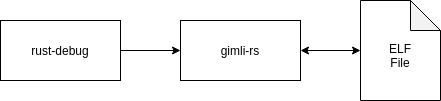
\includegraphics[width=1.0\textwidth]{rust_debug.png}
	\caption{A diagram showing the relation between the \emph{ELF} file and the two libraries \emph{rust-debug} and \emph{gimli-rs}.}
	\label{fig:rustdebug}
\end{figure}


Some of the main functionality that \emph{rust-debug} provides are the following:

\begin{itemize}
  \item Retriving the source file location for funcitons, variables, types and more.
  \item Virtually unwinding the call stack.
  \item Evaluating variables.
  \item Translating soruce file line number to the nearest machine code address.
\end{itemize}

There is more functionalities that \emph{rust-debug} provides but they are not notisable.



\subsubsection{Retriving Source File Location}
% Explain the evaluation of source informaiton % TODO
Some of the \glspl{die} in \gls{DWARF} have attributes that starts with \emph{DW\_AT\_decl\_}.
These attributes contain infomation on where in the source file the \gls{die} was decleard.
This include file path, line number and column number.
The library \emph{rust-debug} has a function for retrieving the value of all these attributes from a given \gls{die}.


The attribute  \emph{DW\_AT\_decl\_file} wich contain the file path of where the \gls{die} was decleard has a file indexd as it's value.
Every compliation unit has a line number information table that contain file paths which are index.
Thus the \emph{rust-debug} libary will search for the maching index in the table to find the file path.
Finding the line and column number does not require any lookup. there attributes contain the value.


\subsubsection{Accessing Memory And Registers}
% Explain the evaluation part. % TODO
% Explain the stored target memory and registers
One of the requirements for evaluating the value of a variable is access to the registers and memory of the debug target.
\emph{rust-debug} does not have that functionality because it should be hardware independet as much as possible.
Intead the library uses a data structure which contain the values of the registers and memory.
This keeps the library hardware independent.
The data structure also has some function for reading and adding values.


The register and memory data structture is used as an argument to the functions in the library.
If a value is missing the called function will return a values that says which value is missing.
Then the user of the library can read that value from the debugged target and add it to the data structure.
Now the funciton can be called again and there are no more missing values it will return the requested value.
Otherwise the user has to reapet the same process.


\subsubsection{Evaluating Variables}
% Explain the evaluation of vairbles.
The \emph{rust-debug} library has a structure called \emph{VariableCreator}, it takes a reference to a \gls{DWARF} unit and \gls{die}.
The \gls{die} has to be one that represents a variable.
When the data strucute is created it will extrac some important informantion about the variable from the \gls{die}.


A constucuted \emph{VariableCreator} struct has a method for evaluating the value of the variable that requires the register and meory data structure.
This method evalutes the variable as describe in section \ref{sec:evaluate-variable} and the \gls{DWARF} specification \cite{dwarf}.
The return value of the method is a enum that is used for telling the user if a value is missing from the register and memory data structure or not.
Then there is another method for retriving the variable information containing the evaluated value.
The variable information contains the following:

\begin{itemize}
  \item The variables name.
  \item The variables type
  \item The variables location in the source file.
  \item The locations of the variables value in registers and memory.
  \item The evaluated value of the variable.
\end{itemize}


\subsubsection{Unwinding Call Stack}
% Explain the evaluation of call stack % TODO
% Explain the evaluation of stackframe 


Using the call stack result each call frame can be used to create a stack frame.
These stack frames are like the call frames except that they have more information like the function name of the frame, where the function was declared and the value of all the variables.
The way this library  constructs a \emph{StackFrame} struct works the same way as when creating a variable.
Meaning that there is a helper struct for creating the stack frame which requires the memory and register struct as an argument.
This helper struct when created will find the name of the function for this frame and where it was declared, then it will go through all dies that belong to that function to find all the variable dies and store it in a list.
This list of variable dies is then used to evaluate all variables and each entry is removed when evaluated and the result stored in a variables attribute.
Thus if one of the variables requires a value from memory that is not present in the memory and register struct then all the variables already evaluated doesn't need to be evaluated again.
The evaluating of the variables is done in the same way as describe above the only difference is that the registers values is set to be the ones evaluated in the call frame.
Thus adding the value of a register to the memory and register struct won't do anything when evaluating a stack frame.
Then lastly the stack frame can be retrieve using the method \emph{get\_stack\_frame} from the stack frame helper struct.


\subsubsection{Finding Breakpoint Location}
% Explain how to get breakpoint locaiton.
The \emph{rust-debug} library has a function that finds a machine code location using a soruce file locaiton.
This machine code locaiton is the closest one that represents the line in the source code.
The funciton requires a file path and line number, but it also can take a column number.


The mention function works by first finding out which compilation unit contains information on the inputed file path.
It thoes this by looping through all the file entries in the line number information table, for every compilation unit.
Each line number information table entry have rows that each contain informaiton on a line from the source code.
Thus all the rows with the search line numbers are added to a list.
The machine code address of the first element in this list is returnd if no column line was inputed to the function.
Otherwiese it is the one with the closest column number that is reurned.

